\documentclass{article}
\usepackage{graphicx}
\usepackage[margin=2cm, a4paper]{geometry}
\usepackage{setspace}
\usepackage{pdfpages}
\usepackage{float}
\usepackage{amsmath}
\usepackage{fancyvrb}
\usepackage{amssymb}
\usepackage{minted}
\usepackage{enumitem}
\usepackage[colorlinks,linkcolor=blue]{hyperref}


\renewcommand{\contentsname}{Contents}
\renewcommand{\figurename}{Figure}
\renewcommand{\tablename}{Table}
\hypersetup{
    colorlinks=true,
    linkcolor=black,
    filecolor=magenta,      
    urlcolor=blue,
}
\newcommand{\mytitle}{Numerical Method - Homework 2}
\newcommand{\myauthor}{B13902022 Yu-Chi,Lai}

\usepackage{fancyhdr}
\pagestyle{fancy}
\fancyhead{}
\fancyhead[L]{\mytitle}
\fancyhead[R]{\myauthor}

\title{\mytitle}
\author{\textbf{\myauthor}}
\date{}

\begin{document}

\maketitle

\section{}
\subsection{(a)}
In section 3.4, I found: "Trivially, you can also apply a positive operator to a numeric expression: \texttt{int x = +42;} Numeric values are assumed to be positive unless explicitly made negative, so this operator has no effect on program operation"

Hence, the expression 0.0 conveys +0.0 by default. The code and its output is my experiment.
\inputminted[
    frame=lines,
    framesep=2mm,
    baselinestretch=1.2,
    bgcolor=lightgray!10,
    linenos
]{c}{positive_zero.c}
\begin{figure}[H]
    \centering
    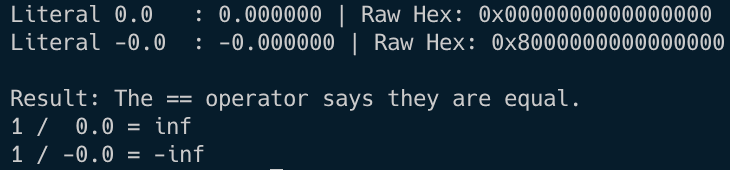
\includegraphics[width=0.5\linewidth]{1a.png}
    \caption{The output}
\end{figure}
\subsection{(b)}
In section 7.12.3.6, there's an \texttt{signbit()} macro in C99 standard (And you should also \texttt{\#include <math.h>}). The \verb|signbit| macro returns a nonzero value if and only if the sign of its argument value is negative.
\subsection{(c)}
We can declare/specify them using unary operators, positive/negative number division by infinity, zero times positive/negative number or the \texttt{copysign()} method in \texttt{<math.h>}. The program below is my experiment:
\inputminted[
    frame=lines,
    framesep=2mm,
    baselinestretch=1.2,
    bgcolor=lightgray!10,
    linenos,
    breaklines
]{c}{1c.c}
\begin{figure}[H]
    \centering
    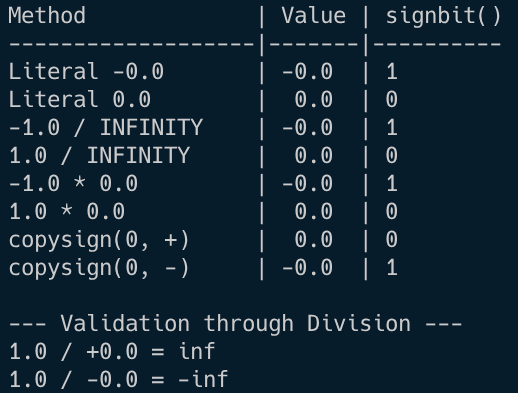
\includegraphics[width=0.5\linewidth]{1c.png}
    \caption{The output of the program above.}
\end{figure}
\subsection{(d)}
We should adopt the first implementation ($(x>y)?x:y$) because if we set $b=-0.0$, the returned value of the first implementation is +0.0=0.0 (Hence, $c=-\infty<0$) while the second implementation gives -0.0 (Hence, $c=+\infty>0$). We can use the program below to prove our claim. 
\inputminted[
    frame=lines,
    framesep=2mm,
    baselinestretch=1.2,
    bgcolor=lightgray!10,
    linenos
]{c}{max_test.c}
\begin{figure}[H]
    \centering
    
\includegraphics[width=0.2\linewidth]{1d.png}
    \caption{The output.}
\end{figure}
\section{}
\subsection*{(i)}
Because I don't have matlab locally, I use GNU octave to implement everything.

\noindent \textbf{No loop (vectorized) version:}
\inputminted[frame=lines,framesep=2mm,baselinestretch=1.2,linenos]{octave}{chol_vectorized.m}
\noindent \textbf{One-level loop version:}
\inputminted[frame=lines,framesep=2mm,baselinestretch=1.2,linenos]{octave}{chol_onelevel.m}
\noindent \textbf{Two-level loop version:}
\inputminted[frame=lines,framesep=2mm,baselinestretch=1.2,linenos]{octave}{chol_twolevel.m}
\subsection*{(ii)}
In my code, I generate a random $n\times n$ matrix $X$, and then we get a symmetry matrix $XX^T$ which is also positive semi-definite. The reason why it is can be shown below:
\begin{align*}
    \text{Let }A=XX^T \\
    A^T=(XX^T)^T=(X^T)^TX^T=XX^T=A \\
    \forall v\in\mathbb{R}^n,v\ne \vec{0},v^TAv=v^TAA^Tv=(A^Tv)^T(A^Tv)\ge 0 
\end{align*}
And then by adding a $n\times n$ identity matrix times a positive constant, we can ensure that $v^T(A+nI)v=v^TAv+nv^TIv>0$, i.e., positive definite, without breaking the symmetry. The below is my code:
\inputminted[frame=lines,framesep=2mm,baselinestretch=1.2,linenos]{octave}{generate_spd.m}
\begin{figure}[H]
    \centering
\includegraphics[width=0.6\linewidth]{verify.png}
    \caption{The correctness of my three implementations of cholesky factorization (proved by built-in \texttt{chol()})}
\end{figure}
\subsection*{(iii)}
I used meow1 (with GPU) in CSIE workstation, and the code for testing and its result are shown as below. For small to medium matrix sizes (such as $n=10,100,1000$), the vectorized version is faster than the one-loop version, while the two-loop version is much slower. However, for $n=4000$, the performance order changes to one-loop $>$ vectorized $>$ two-loop. Therefore, the fastest method depends on matrix size, and for very large matrices the one-loop version can outperform the vectorized implementation.
\inputminted[frame=lines,framesep=2mm,baselinestretch=1.2,linenos, breaklines]{octave}{test_time.m}
\begin{figure}[H]
    \centering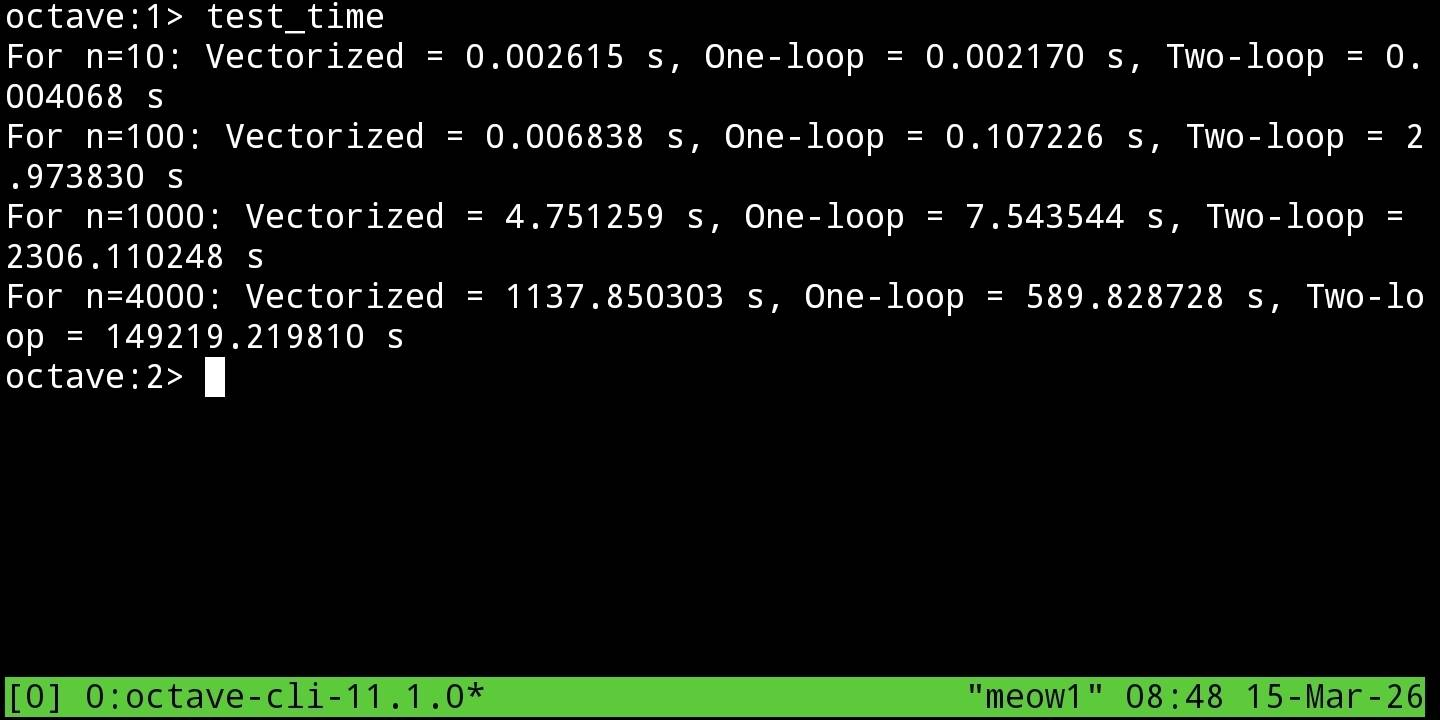
\includegraphics[width=0.7\linewidth]{tic.png}
    \caption{The results}
\end{figure}
\subsection*{(iv)}
I found that the vectorized implementation significantly outperformed the looped versions because it avoids the interpreter overhead associated with element-by-element processing. 

According to the Octave manual, vectorization allows the program to bypass high-level interpretation and utilize optimized internal C++, C, or Fortran libraries that leverage hardware vector instructions. The goal of vectorization is to write code that is making loops less (like for and while), instead, use whole array operations which is more efficient.

For small to medium matrices, this approach can achieve the typical speedup of Octave's matrix-oriented design, because vectorized operations call optimized low-level BLAS/LAPACK routines and reduce interpreter overhead.

However, for very large matrices (for example, $n=4000$ in my test), the vectorized version became slower than the one-loop version. This is mainly due to memory pressure: the vectorized rank-1 updates create large temporary arrays repeatedly, which increases memory traffic and cache misses. The one-loop version updates matrix columns directly, which is more cache-friendly and reduces temporary allocation cost.

The two-loop version is still the slowest because it performs element-by-element updates, so loop control and interpreter overhead accumulate heavily. In summary, the Octave results are consistent with the MATLAB analysis: vectorization is best for smaller sizes, while one-loop can be better for large-scale problems where memory bandwidth becomes the bottleneck.
% \subsection*{(v)}

\section{Matlab implementation (2(v))}
The behind-scene theory and technique I used in this part is almost the same as that in octave, so I don't further explain how these codes work here.
\subsection{Symmetric positive difinite matrix}
\begin{figure}[H]
\inputminted[frame=lines,framesep=2mm,baselinestretch=1.2,linenos, breaklines]{matlab}{matlab/generate_spd.m}
\caption{The function for generating Symmetric positive difinite matrix (using MATLAB)}
\end{figure}
\begin{figure}[H]
    \centering
    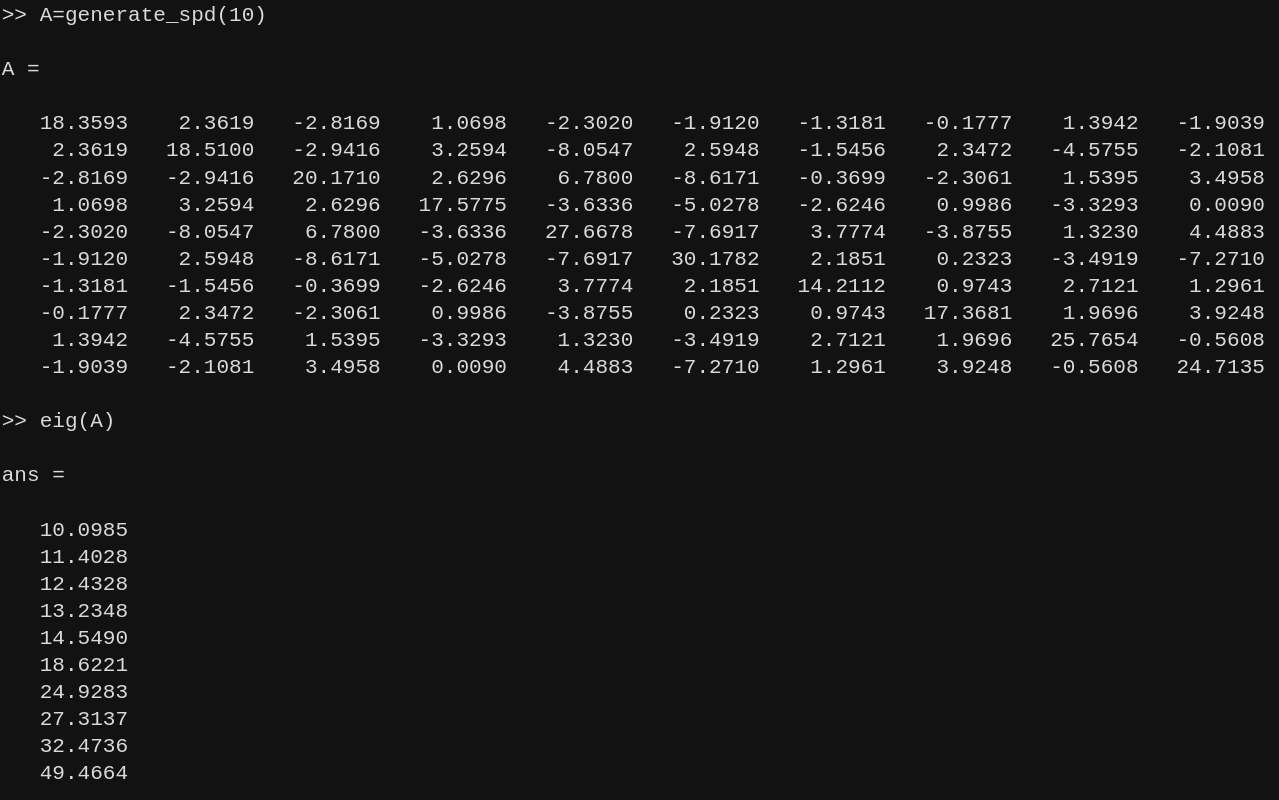
\includegraphics[width=0.7\linewidth]{matlab_pic/spd.png}
    \caption{By using \texttt{eig()} function, we can found all eigenvalues are positive for real.}
\end{figure}
\subsection{Cholesky decomposition (3 methods)}
\begin{figure}[H]
\inputminted[frame=lines,framesep=2mm,baselinestretch=1.2,linenos, breaklines]{matlab}{matlab/chol_vectorized.m}
\caption{Vectorized Cholesky decomposition implementation (using MATLAB)}
\end{figure}
\begin{figure}[H]
\inputminted[frame=lines,framesep=2mm,baselinestretch=1.2,linenos, breaklines]{matlab}{matlab/chol_oneloop.m}
\caption{One-loop Cholesky decomposition implementation (using MATLAB)}
\end{figure}
\begin{figure}[H]
\inputminted[frame=lines,framesep=2mm,baselinestretch=1.2,linenos, breaklines]{matlab}{matlab/chol_twoloop.m}
\caption{Two-loop Cholesky decomposition implementation (using MATLAB)}
\end{figure}
\begin{figure}[H]
    \centering
    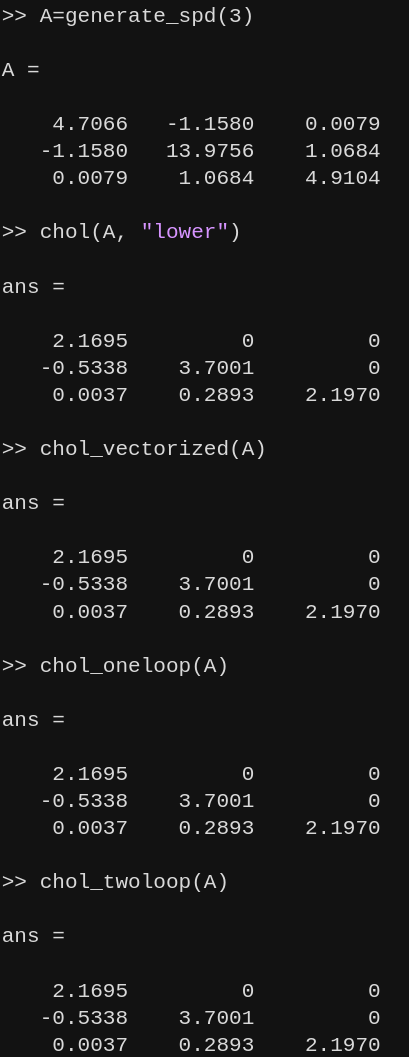
\includegraphics[width=0.4\linewidth]{matlab_pic/verify.png}
    \caption{The correctness of my three codes by \texttt{chol()} function}
\end{figure}
\subsection{Efficiency analysis}
I tested the three Cholesky factorization implementations in MATLAB (using the MATLAB Online free plan) for $n \in \{10, 100, 1000, 2000, 4000\}$. The timing results revealed a significant shift in performance efficiency as the matrix size $n$ increased.

For small to medium matrices ($n \le 1000$), the \textbf{Vectorized} version was the fastest. Because the matrices are relatively small, the memory required to perform the operations easily fits into the CPU's high-speed L1/L2 cache. Consequently, the vectorized code fully benefits from MATLAB's underlying highly-optimized numerical libraries (such as BLAS and LAPACK) and bypasses the interpreter overhead associated with loop management.

However, for massive matrices ($n = 4000$), the performance inverted entirely: the \textbf{One-loop} version was the fastest ($\approx 37.1$ s), the \textbf{Two-loop} version was second ($\approx 65.8$ s), and the \textbf{Vectorized} version was the slowest by a wide margin ($\approx 113.7$ s). This occurs due to the interplay between memory bandwidth and compiler optimization:

\begin{itemize}
    \item \textbf{Why One-loop outperforms Vectorized (The Memory Bottleneck):} The vectorized update formula computes the outer product $vv^T$, generating a massive temporary matrix (up to $4000 \times 4000$) during every single iteration. Continuously allocating, writing, and clearing this large block of memory forces the CPU to constantly fetch data from the slower main RAM, causing severe cache thrashing. The One-loop version avoids this by updating the matrix column-by-column. A single column easily fits into the CPU cache, eliminating the memory bandwidth bottleneck.
    
    \item \textbf{Why One-loop outperforms Two-loop (JIT and Interpreter Overhead):} While both looped versions avoid creating massive temporary matrices, the Two-loop updates the matrix element-by-element. Even though modern MATLAB features a Just-In-Time (JIT) compiler to accelerate loops, managing the loop conditions and array bounds for millions of individual $A(i,j)$ elements still introduces noticeable computational overhead. The One-loop version hits the optimal "sweet spot": it processes cache-friendly chunks of data (columns) while still utilizing low-level, optimized vector operations for each column update.
\end{itemize}
\begin{figure}[H]
\inputminted[frame=lines,framesep=2mm,baselinestretch=1.2,linenos, breaklines]{matlab}{matlab/test_time_matlab.m}
\caption{Performance testing script for Matlab implementations (using MATLAB)}
\end{figure}
\begin{figure}[H]
    \centering
    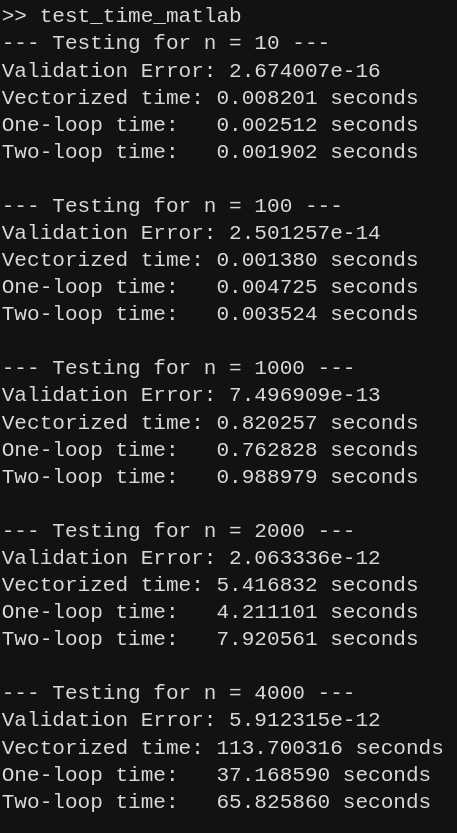
\includegraphics[width=0.4\linewidth]{matlab_pic/tt.png}
    \caption{The execution time tests for Vectorized, One-loop, Two-loop version of Cholesky decomposition}
\end{figure}


\end{document}
% how to display codes?
% \begin{minted}[frame=lines,framesep=2mm,baselinestretch=1.2,linenos,breaklines]{python}
% \end{minted}

% how to display images?
% test